
\medskip

On souhaite rénover une salle de bain qui a la forme d’un parallélépipède rectangle. Il faut coller du papier peint sur les quatre murs. On n’en colle pas sur la porte, ni sur la fenêtre.
	
Voici un schéma de la salle de bain, les dimensions sont exprimées en mètre :
	
\begin{center}
	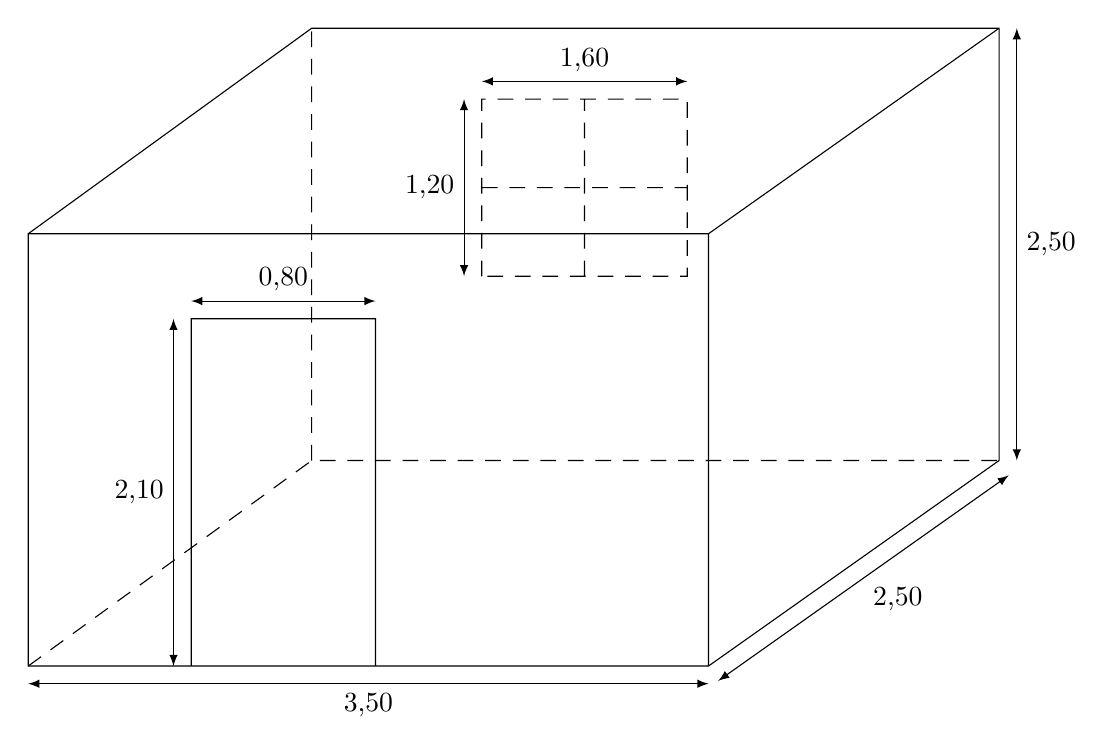
\begin{tikzpicture}[x=0.9cm,y=0.9cm,> = latex]
		\draw  (0,0) rectangle (9.6,6.1)
			   (2.3,0) rectangle (4.9,4.9)	
			   (0,6.1)--(4,9)--(13.7,9)--(13.7,2.9)--(9.6,0)
			   (9.6,6.1)--(13.7,9);
		\draw[dash pattern=on 2mm off 1.5mm] 
				(0,0)--(4,2.9)--(13.7,2.9)
				(4,2.9)--(4,9)
				(6.4,5.5) rectangle (9.3,8)
				(7.85,5.5)--(7.85,8)
				(6.4,6.75)--(9.3,6.75);
		\draw[<->, shift={(0,-0.25)}] (0,0)--(9.6,0)
		node[below,pos=0.5]{3,50};
		\draw[<->, shift={(-57:0.25)}] (9.6,0)--(13.7,2.9)
		node[below right,pos=0.5]{2,50};
		\draw[<->, shift={(0.25,0)}] (13.7,2.9)--(13.7,9)
		node[right,pos=0.5]{2,50};
		\draw[<->, shift={(-0.25,0)}] (2.3,0)--(2.3,4.9)
		node[left,pos=0.5]{2,10};
		\draw[<->, shift={(0,0.25)}] (2.3,4.9)--(4.9,4.9)
		node[above,pos=0.5]{0,80};
		\draw[<->, shift={(-0.25,0)}] (6.4,5.5)--(6.4,8)
		node[left,pos=0.5]{1,20};
		\draw[<->, shift={(0,0.25)}] (6.4,8)--(9.3,8)
		node[above,pos=0.5]{1,60};
	\end{tikzpicture}
\end{center}
	
	On dispose des informations suivantes :
	
	\fbox{\rule[-2.1cm]{0mm}{4.4cm}\begin{minipage}{0.53\linewidth}
			Prix du papier peint :
			
			\begin{itemize}[label=\textbullet,leftmargin=*]
				\item le papier peint est vendu au rouleau entier ;
				
				\item un rouleau coûte 16,95 \euro{};
				\item un rouleau permet de recouvrir 5,3 m$^2$.
			\end{itemize}
			\emph{Conseil du vendeur :} 
			
			prévoir 1 rouleau de papier peint en plus afin de compenser les pertes liées aux découpes.
	\end{minipage}}
	\hfill
	\fbox{\rule[-2.1cm]{0mm}{4.4cm}\begin{minipage}{0.42\linewidth}
		Prix de la colle :
		\begin{itemize}[label=\textbullet,leftmargin=*]
			\item la colle est vendue au pot entier ;
			\item un pot a une masse de 0,2 kg;
			\item un pot coûte 5,70 \euro{}.
		\end{itemize}
				\emph{Conseil du vendeur :}
		
		compter 1 pot de colle pour 4 rouleaux de papier peint.		
	\end{minipage}}

	\begin{enumerate}
		\item Montrer que la surface à recouvrir de papier peint est de 26,4 m$^2$.
		
		\item Calculer le prix, en euro, d’un mètre carré de papier peint.
		Arrondir au centime d'euro.
		
		\item Si on suit les conseils du vendeur, combien coûtera la rénovation de la salle de bain ?
		
		\item Le jour de l'achat, une remise de 8 \% est accordée.
		
		Quel est le prix à payer après remise ? Arrondir au centime d'euro.
	\end{enumerate}

